\subsection{Метод Ньютона решения уравнений и систем уравнений}
\subsubsection{Метод Ньютона решения уравнений}

Метод Ньютона относится к градиентным методам. В данном классе методов для нахождения корня используется значение производной.
Дано нелинейное уравнение:
\begin{center}
\begin{equation}
	\label{eq:newton_base}
	f(x) = 0
\end{equation}
\end{center}

Найти корень в интервале   с заданной точностью.
Данный метод основан на замене функции ${f(x)}$, на каждой итерации поиска касательной, проведенной к этой функции. Пересечение касательной с осью ${x}$
дает приближение корня (рисунок \ref{pic:newton_method}).
 
\begin{figure}[H]
	\center\scalebox{0.7}{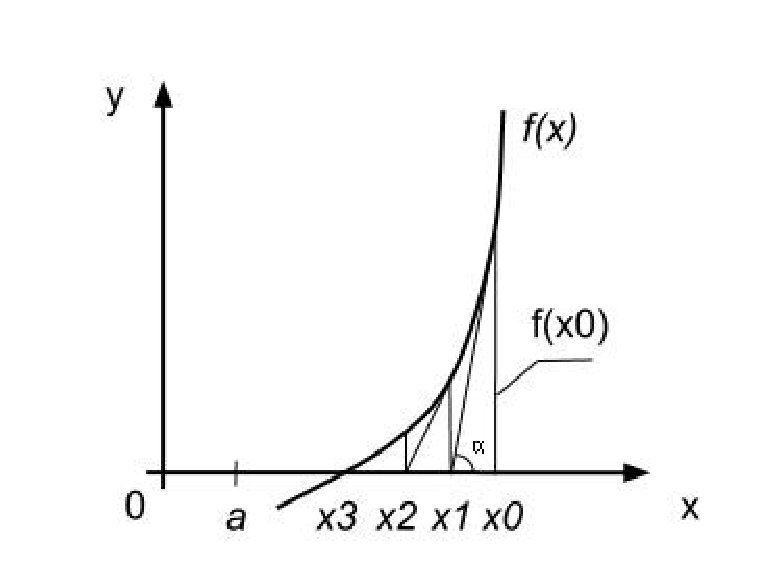
\includegraphics[width=1\linewidth]{newton_base.eps}}
	\caption{Метод Ньютона}
	\label{pic:newton_method}
\end{figure}

Выберем начальную тучку ${x_0=b}$. Находим значение функции в этой точке и восстанавливаем к ней касательную, пересечение которой с осью ${x}$
дает нам первое приближение корня ${x_1}$.  Метод обеспечивает быструю сходимость, если выполняется условие:
\begin{center}
\begin{equation}
	\label{eq:newton_base_1}
	f(x_0)f''(x_0) > 0
\end{equation}
\end{center}

Итерационный процесс схождения к корню выполняется по рекуррентной формуле:
\begin{center}
\begin{equation}
	\label{eq:newton_eq}
	x_{n+1} = x_n - \frac{f(x_n)}{f'(x_n)}
\end{equation}
\end{center}

Итерационная процедура продолжается до выполнения условия:
\begin{center}
\begin{equation}
	\label{eq:newton_eq_bound}
	\frac{f(x_n)}{f'(x_n)} \leq \epsilon
\end{equation}
\end{center}
где ${\epsilon}$ - заданная точность.

%%%%%%%%%%%%%%%%%%%%%%%%%%%%%
\subsubsection{Метод Ньютона решения систем уравнений}
% http://e-lib.gasu.ru/eposobia/metody/R_2_3.html
% http://www.intuit.ru/department/calculate/intromathmodel/4/intromathmodel_4.html
Рассмотрим систему двух уравнений:
\begin{center}
\begin{equation}
	\label{eq:newton_system}
		\begin{cases}
			f_1(x_1, x_2) = 0 \\
			f_2(x_1, x_2) = 0.
		\end{cases}
\end{equation}
\end{center}

Решение данной системы уравнений по методу Ньютона будет задаваться формулами:
\begin{center}
\begin{eqnarray}
	\label{eq:newton_system_2}
		\left[ \begin{array}{c}
			x_1^{n+1} \\
			x_2^{n+1}
		\end{array} \right]
	=
		\left[ \begin{array}{c}
			x_1^{n} \\
			x_2^{n}
		\end{array} \right]
	- J^{-1} (x_1^n, x_2^n)
		\left[ \begin{array}{c}
			f_1(x_1^n, x_2^n) \\
			f_2(x_1^n, x_2^n)
		\end{array} \right]
\end{eqnarray}
\end{center}
где 
\begin{center}
\begin{eqnarray}
	\label{eq:newton_system_3}
	J(x_1^n, x_2^n) = 
		\left[ \begin{array}{cc}
			\frac{\partial f_1 (x_1^n, x_2^n)}{\partial x_1} & \frac{\partial f_1 (x_1^n, x_2^n)}{\partial x_2} \\
			\frac{\partial f_2 (x_1^n, x_2^n)}{\partial x_1} & \frac{\partial f_2 (x_1^n, x_2^n)}{\partial x_2}
		\end{array} \right]
\end{eqnarray}
\end{center}
а ${(x_1^0, x_2^0)}$ - начальное приближение.

Критерием окончания итерационного алгоритма Ньютона для вычисления корня системы уравнений с заданной точностью ${\epsilon}$ может служить выражение:
\begin{center}
\begin{equation}
	\label{eq:newton_system_4}
	\|x^{k+1} - x^k\| \leq \epsilon
\end{equation}
\end{center}



\newpage
